\documentclass[a4paper,10pt]{report}

\usepackage[utf8]{inputenc}

\usepackage{graphicx,url}
\usepackage[brazil]{babel}
\usepackage{float}
\usepackage{listings}
\usepackage{subfigure}
\usepackage{amsmath}
\usepackage{xspace}

\newcommand{\ferramenta}{\texttt{MSN - Resolução de Sistemas de Equações Lineares}\xspace}

\begin{document}

\title{Manual da ferramenta \ferramenta}
\author{MSN 2008.2}

\bibliographystyle{plain}

\maketitle

\tableofcontents

\chapter{Introdução}
\label{intro}

A ferramenta \ferramenta foi desenvolvida para a disciplina de \textit{Métodos de Software Numérico} ministrada pelo professor Eustáquio Rangel na \textit{Universidade Federal de Campina Grande} pelo \textit{Departamento de Sistemas e Computação}. Tendo como desenvolvedores toda a equipe de alunos da disciplina, e usando a linguagem de programação Java, a ferramenta busca resolver sistemas de equações lineares usando diversos métodos pesquisados e discutidos em sala de aula.

Este documento descreve um manual de uso da ferramenta. No capítulo~\ref{instalacao}, é descrita a instalação e uso inicial da ferramenta. O capítulo\ref{resolucao} descreve o funcionamento da ferramenta: como usá-la para a resolução de sistemas lineares, incluindo um embasamento teórico dos procedimentos realizados. Por fim, o capítulo~\ref{desenvolvedor} descreve um pequeno manual para o desenvolvedor, com as decisões arquiteturais do projeto e uma descrição do funcionamento e organização do código da mesma.

\section{Licença}

Esta ferramenta está liberada sob a licença GPL 2.0\cite{gpl}.

\section{Código Fonte}

O acesso ao código fonte, documentação e informações sobre o projeto podem ser acessadas no site: \texttt{http://code.google.com/p/msn-sistemas-lineares/}. Para acessar o código fonte, basta usar o SVN~\cite{svn}, localizado no endereço: \texttt{http://msn-sistemas-lineares.googlecode.com/svn/trunk/}.

\section{Equipe de Desenvolvedores}

\begin{itemize}
 \item Adauto Trigueiro
 \item Alan Farias
 \item Anderson Pablo
 \item Dayane Gaudencio
 \item Diego Melo Gurjão
 \item Everton Leandro
 \item Hugo Marques
 \item Jackson Porciuncula
 \item João Felipe Ouriques
 \item José Wilson
 \item José Gildo
 \item Leonardo Ribeiro Mendes
 \item Rafael Dantas
 \item Ricardo Araújo
 \item Roberta Guedes
 \item Rodrigo Pinheiro
 \item Theo Alves
\end{itemize}

\chapter{Instalação}
\label{instalacao}

\section{Dependências}

A ferramenta executa sobre a plataforma Java, aproveitando todas as suas
vantagens como, por exemplo, a independência de sistema operacional, desde que
exista uma máquina virtual compatível com tal sistema.

\section{Execução}

Utilizando o jar disponibilizado, para executar o usuário necessita do comando:

\texttt{java -jar nome\_do\_jar.jar}

Dessa forma a ferramenta não necessita de instalação, trazendo uma vantagem ao
usuário que não tem permissões para instalar aplicativos.

\chapter{Resolução de Sistemas de Equações Lineares}
\label{resolucao}
Esta seção descreve como a ferramenta trabalha para a resolução de sistemas de equações lineares. Para contextualizar o leitor, é importante enteder como são definidos tais sistemas. Esta base é usada posteriormente na explicação dos métodos de resolução de sistemas de equações lineares.

Todo sistema de equações lineares representa uma composição de equações lineares, como mostra o exemplo a seguir:

\[
\begin{array}{cccccccc}
a_{1,1}x_{1} & + & a_{1,2}x_{2} & \cdots & + & a_{1,n}x_{n} & = & b_{1}\\
a_{2,1}x_{1} & + & a_{2,2}x_{2} & \cdots & + & a_{2,n}x_{n} & = & b_{2}\\
\vdots  & & \vdots  &  \ddots & & \vdots &  & \vdots  \\
a_{m,1}x_{1} & + & a_{m,2}x_{2} & \cdots & + & a_{m,n}x_{n} & = & b_{m}
\label{arr:sistema}
\end{array}
\]

É possível obter uma matriz representando os coeficientes das equações lineares que compõe o sistema. Esta matriz é da forma:

\[
A = \left[ \begin{array}{cccc}
a_{1,1} & a_{1,2} & \cdots & a_{1,n} \\
a_{2,1} & a_{2,2} & \cdots & a_{2,n} \\
\vdots  & \vdots & \ddots & \vdots \\
a_{m,1} & a_{m,2} & \cdots & a_{m,n}
\label{arr:coeficientes}
\end{array}\right]
\]

Dois outros vetores também são obtidos a partir das equações lineares do sistema inicial. O primeiro vetor representa as incógnitas do sistema:

\[
x = \left[ \begin{array}{c}
x_{1} \\
x_{2} \\
\vdots \\
x_{m}
\label{arr:icognitas}
\end{array}\right]
\]

E o segundo vetor composto pelos termos independentes do sistema:

\[
b = \left[ \begin{array}{c}
b_{1} \\
b_{2} \\
\vdots \\
b_{m}
\label{arr:termos}
\end{array}\right]
\]

Observe que ao multiplicar cada linha de $A$, ou seja, da \textit{matriz dos coeficientes}, pelo vetor \textit{x} (incógnitas do sistema), obtêm-se como resultado cada valor do vetor dos termos independentes, $b$. Assim, o sistema original pode ser representado por $A$, $x$ e $b$ como descrito na equação~\ref{eqn:sistemas}.

\begin{equation}
Ax = b
\label{eqn:sistemas}
\end{equation} 

Uma representação útil do sistema, a ser usado em alguns métodos a serem apresentados é a da matriz expandida do sistema. Esta matriz $A_{expand}$ é definida como a matriz dos coeficientes acrescida ao vetor dos termos $b$. Ou seja:

\[
A_{expand} = \left[ \begin{array}{cccccc}
a_{1,1} & a_{1,2} & \cdots & a_{1,n} & \vline & b_{1} \\
a_{2,1} & a_{2,2} & \cdots & a_{2,n} & \vline & b_{2} \\
\vdots  & \vdots & \ddots & \vdots & \vline & \vdots \\
a_{m,1} & a_{m,2} & \cdots & a_{m,n} & \vline & b_{m} 
\label{arr:coeficientes}
\end{array}\right]
\]

Visualizando o sistema como uma operação matricial, é possível identificar propriedades do sistema a partir das proriedades da matriz de coeficientes da equação. Em especial, a matriz $A$ de tamanho $m \times n$, apresenta $m$ incógnitas e $n$ equações lineares.

Durante a resolução de tal sistema, três possibilidades de resultados estão descritos na tabela~\ref{tab:sistemas}.

\begin{table}[h]
\centering
\caption{Possíveis Resultados de um Sistema}
        \begin{tabular}{|c|p{2in}|}
        \hline
        \textbf{Tipo} & \textbf{Descrição} \\ \hline
        \textbf{Possível e Determinado} & O sistema é possível e apresenta uma única solução \\ \hline
        \textbf{Possível e Indeterminado} & O sistema é possível, mas não apresenta uma única solução \\ \hline
        \textbf{Impossível} & O sistema não tem solução \\ \hline
        \end{tabular}
\label{tab:sistemas}
\end{table} 

Num sistema onde $m > n$, ou seja, há mais incógnitas do que equações, não é possível determinar uma solução única para o sistema: cada equação representa um vetor no espaço de $m$ dimensões, e a solução única só é possível quando a intereseção de todas as equações forma um ponto no espaço. Note que tal sistema também poderia não ter solução: basta considerar o exemplo de quando dois vetores são paralelos no espaço, assim, não apresentando pontos comuns de interseção.

Quando $m < n$, o sistema possivelmente não apresenta soluções. Fazendo um análogo com a interpretação espacial de um sistema de equações lineares, $m$ equações possivelmente apresentará como intereseção um único ponto no espaço. A adição de uma nova equação pode não interceptar este mesmo ponto, fazendo com o que o sistema se torne impossível de ser solucionado. Observe que é possível que a nova equação ainda permita que o sistema tenha uma única solução: basta que este vetor intercepte o mesmo único ponto que os demais vetores no espaço.

Devido as possíveis interpretações de um sistema em que $m \neq n$, a ferramenta limita-se apenas em explorar os sistemas homogêneos. Nestes sistemas $m = n$. Esta restrição permite explorar a matriz de entrada do sistema, verificado ao usuário qual a classificação do tipo do sistema (possível e determinado, possível e indeterminado ou impossível).

Para realizar esta verificação, utiliza-se de parte da regra de Cramer~\cite{cramer}. Em especial, considerando que a matriz $A$ tem tamanho $n \times n$, então:

\[
D \equiv \left| \begin{array}{cccc}
a_{1,1} & a_{1,2} & \cdots & a_{1,n} \\
a_{2,1} & a_{2,2} & \cdots & a_{2,n} \\
\vdots  & \vdots & \ddots & \vdots \\
a_{n,1} & a_{n,2} & \cdots & a_{n,n}
\label{arr:detcoeficientes}
\end{array}\right|
\]

Ainda, pra cada incógnita existe um $D_{k}$ tal que:

\[
D_{k} \equiv \left| \begin{array}{ccccccc}
a_{1,1} & \cdots & b_{1} & a_{1,k+1} & \cdots & a_{1,n}\\
\vdots  & \ddots & \vdots & \vdots  & \ddots & \vdots \\
a_{n,1} & \cdots & b_{n} & a_{n,k+1} & \cdots & a_{n,n}
\label{arr:detcoeficientesk}
\end{array}\right|
\]

Assim, considerando $D$ e $D_{k}$, é possível determinar o tipo de resolução do sistema, como mostra as condições da tabela~\ref{tab:sistemad}.

\begin{table}[h]
\centering
\caption{Condições para Indentificação das Soluções de um Sistema}
        \begin{tabular}{|c|c|}
        \hline
        \textbf{Tipo} & \textbf{Condição} \\ \hline
        \textbf{Possível e Determinado} & $D \neq 0$ \\ \hline
        \textbf{Possível e Indeterminado} & $D = 0$, $\forall k, D_{k} = 0$ \\ \hline
        \textbf{Impossível} & $D = 0$, $\exists k | D_{k} \neq 0$ \\ \hline
        \end{tabular}
\label{tab:sistemad}
\end{table} 

Assim, considerando a limitação da ferramenta em que apenas sistemas homogêneos são verificados, a ferramenta também verifica se o sistema tem solução possível e determinada, possível e indeterminada, ou se é impossível de ser resolvido. Este cálculo é feito a partir das determinantes do sistema, como apresentado anteriormente.

% \section{Usando a Ferramenta}
% 
% TODO

\section{Métodos de Resolução de Sistemas de Equações Lineares}

Os métodos usados pela ferramenta podem ser classificados como diretos ou iterativos. Nos métodos diretos, são conhecidos os números de passos e o procedimento para se obter um vetor de solução do sistema. Enquanto nos métodos iterativos, a solução é refinada até que seja obtido um vetor que satisfaça à precisão definida.

São métodos diretos:
\begin{itemize}
 \item Método da Eliminação de Gauss
 \item Método da Eliminação de Gauss-Jordan
 \item Método da Decomposição LU e SVD
 \item Método da Decomposição de Cholesky e QR
\end{itemize}

São métodos iterativos:
\begin{itemize}
 \item Método de Gauss-Jacobi
 \item Método de Gauss-Siedel
\end{itemize}

As soluções obtidas pelos métodos diretos são refinadas até atingirem um critério definido pelo usuário. Considerando que $x$ representa um vetor de soluções, idealmente:

\[
b - Ax = 0
\]

Entretanto, pelos erros associados as operações numéricas do software, é possível que se obtenha um resíduo $r$ no cálculo desta solução:

\begin{equation}
b - Ax = r
\label{residuo}
\end{equation}

Para amenizar o resíduo, procura-se um vetor de correção $c$ tal que:

\[
\begin{array}{c}
A(x+c) - b = 0 \\
Ax + Ac - b = 0 \\
Ax - b + Ac = 0 \\
Ac = b - Ax \\
\end{array}
\]

Aplicando a equação~\ref{residuo}:

\begin{equation}
Ac = r
\label{residuofinal}
\end{equation}

Basta resolver a equação\ref{residuofinal} para obter um novo vetor de soluções $x^{1}$ tal que $x^{1} = x + c$. Esta nova solução pode ser novamente refinada até que o vetor de resíduo satisfaça os critérios definidos pelo usuário.

\subsection{Método da Eliminação de Gauss com e sem pivoteamento}

O método da eliminação de Gauss faz uso de três operações básicas sobre a matriz expandida do sistema que não altera a solução do mesmo:

\begin{itemize}
 \item Multiplicação de uma equação (linha) por uma constante não nula
 \item Soma do múltiplo de uma equação a outra
 \item Troca de posição de duas ou mais equações
\end{itemize}

O método utiliza de tais operações na busca de uma matriz triangular, isto é, na forma:

\[
A_{expand} = \left[ \begin{array}{cccccc}
\delta_{1,1} & \delta_{1,2} & \cdots & \delta_{1,n} & \vline & b_{1} \\
0 & \delta_{2,2} & \cdots & \delta_{2,n} & \vline & b_{2} \\
\vdots  & \vdots & \ddots & \vdots & \vline & \vdots \\
0 & 0 & \cdots & \delta_{m,n} & \vline & b_{m} 
\label{arr:triangular}
\end{array}\right]
\]

Para se obter esta matriz, considere-se este exemplo trivial:

\[
Exemplo_{expand} = \left[ \begin{array}{cccc}
a_{1,1} & a_{1,2} & \vline & b_{1} \\
a_{2,1} & a_{2,2} & \vline & b_{2}
\label{arr:triangularexemplo}
\end{array}\right]
\]

Para anular o elemento $a_{2,1}$, a segunda linha ($L_{2}$) é susbtituída por $a_{2,1}/a_{1,1} \times L_{1} - L_{2}$, onde $L_{1}$ representa a primeira linha. Ao realizar tal operação o termo $a_{2,1}$ na matriz  $Exemplo_{expand}$ é anulado. O algoritmo de triangularização da matriz irá operar em diagonal, trocando as linhas que apresentem um valor nulo na diagonal por alguma linha abaixo que possua um valor não-nulo na mesma coluna, e, a partir disto, anulando todos os coeficientes abaixo do elemento da diagonal atual.

A partir da matriz resultante de tal operação, o cálculo da solução é direto: basta resolver recursivamente da última linha para primeira o valor de cada incógnita.

O uso de um pivô determina que o sistema fará a escolha da linha de referência para triangularizar a matriz de acordo com o maior elemento existente da coluna. A linha com o maior elemento, passa a ser a linha cuja diagonal da matriz irá possuir tal elemento nesta coluna. Ao escolher tal pivô, as operações usam como referência um valor maior, o que permite diminuir os erros gerados pelas operações de ponto flutuante do software.

\subsection{Método da Eliminação de Gauss-Jordan com e sem pivoteamento}

No método de Gauss-Jordan, deseja-se obter uma matriz expandida equivalente ao sistema original, onde os coeficientes apresentam em toda diagonal elementos não-nulos. Este método complementa o método de eliminação de Gauss apresentado anteriormente, eliminando a etapa da resolução recursiva da matriz triangular, pois o sistema estará na forma:

\[
A_{expand} = \left[ \begin{array}{cccccc}
\delta_{1,1} & 0 & \cdots & 0 & \vline & \beta_{1} \\
0 & \delta_{2,2} & \cdots & 0 & \vline & \beta_{2} \\
\vdots  & \vdots & \ddots & \vdots & \vline & \vdots \\
0 & 0 & \cdots & \delta_{m,n} & \vline & \beta_{m} 
\label{arr:triangular}
\end{array}\right]
\]

Onde a solução é imediata: $x_{1} = \beta_{1}/\delta_{1,1}$.

Para obter esta matriz, o método inicia triangularizando a matriz e, em seguida, tomando a última linha, como referência elimina todos os elementos da última coluna dos coeficientes da matriz. Em seguida, repete o processo para a penúltima linha e assim sucessivamente.

\subsection{Método da Decomposição LU e SVD}

\subsubsection{Decomposição LU}

A resolução do método da decomposição LU se baseia na decomposição da matriz $A$ de $A.x = b$ em duas outras matrizes $L$ e $U$:

\begin{equation*}
A = L.U
\end{equation*}

Onde $L$ é uma matriz triagular inferior com diagonal unitária, ou seja, todos elementos acima da diagonal são nulos e os da diagonal são iguais a 1; e $U$ é uma matriz triangular superior, onde todos os elementos abaixo da diagonal principal são nulos, de forma que: 

\begin{equation*}
LU.x = b
\end{equation*}

Dessa forma, a resolução do sistema $A.x = b$ se reduz à resolução de dois sistemas triangulares: $U.x = y$ e $L.y = b$ . As matrizes L e U podem ser obtidas usando o processo de Gauss, onde a matriz U é a matriz resultante do processo e a matris L é composta dos índices usados para multiplicar as linhas no processo e uma diagonal principal unitária.

\subsubsection{Decomposição SVD}

Quando a matriz A é singular, ou seja, não possui inversa (determinante igual a
0 no teste de Cramer), a decomposição SVD pode ser usada. Matrizes $A (M x N)$
tal que $M$ seja maior ou igual a $N$, podem ser decompostas no produto de três
matrizes: $A = U . W . V^{T}$, tal que U é uma matriz coluna ortogonal; W é uma
matriz diagonal com elementos positivos ou nulos (valores singulares); e V é
uma matriz ortogonal.

Se A for uma matriz quadradam então U W e V também o serão. Logo, de acordo com
\cite{press:recipes92} podemos definir x como:

\begin{equation}
x = V . [diag(1/w_j)].(U^T . b)
\end{equation}

Caso $w_j$ seja nulo podemos substituir $1/w_j$ por zero. 

\subsection{Método da Decomposição de Cholesky e QR}

\subsubsection{Decomposição de Cholesky}
Quando a matriz A é simétrica e positiva definida, ou seja $v.A.v > 0 \forall vetor v$, há uma decomposi,ão triangular mais eficiente. A decomposição de Cholesky constrói uma matriz $L$ diagonal inferior tal que $L^{T}$ serve como matriz U, de modo que $L.L^{T} = A$.

Dessa forma a equação da decomposição LU torna-se:

\begin{equation*}
L.L^{T}.x = b
\end{equation*}

\subsubsection{Decomposição QR}

A decomposição QR consiste em decompor a matriz $A$ no produto $QR$ onde R é
uma matriz triangular superior e $Q$ é uma matriz ortogonal, ou seja, $Q.Q^{T}
= 1$. Substituindo na equaçào $Ax = b$ temos que:

\begin{gather*}
Q.R.x = b\\
R.x = Q^{T}.b\\
\end{gather*}

\subsection{Método de Gauss-Jacobi}

O método de Gauss-Jacobi fundamenta-se em resolver a equação:

\begin{equation*}
Ax = b
\end{equation*}

Sabendo que a matriz A pode ser escrita na forma $ A = D + (L + U) $ onde $D$ representa a diagonal, $L$ a matriz estritamente inferior e $U$ a matriz estritamente superior. Substituindo o resultado na equação e isolando a variável $x$ no primeiro membro, temos que:

\begin{equation*}
x^{(k+1)}=D^{-1}[b-(L+U)x^{(k)}]
\end{equation*}

com $k$ sendo o contador de iterações. Assim sendo, uma abordagem iterativa para a equação acima seria:

\begin{equation*}
 x^{(k+1)}_{i}=\dfrac{1}{a_{ii}}(b-\sum_{j \neq i} a_{ij}x^{(k)}_{j})
\end{equation*}

Com o uso dessa equação os termos da matrix na iteração $k+1$ são calculados única e exclusivamente com os valors na iteração $k$. O processo converge quando a matriz é estritamente diagonal dominante, ou seja, o módulo do elemento na diagonal é maior que a soma do módulo de todos os outros elementos (não diagonais) da linha em questão. Mais precisamente:

\begin{equation*}
|a_{ii}| > \sum_{j \neq i}|a_{ij}| ,  \forall i
\end{equation*}

Há alguns casos onde o método converge sem satisfazer a condição anterior, sendo necessário que os elementos na diagonal principal sejam maiores em magnitude que os outros elementos.

\subsection{Método de Gauss-Seidel}

O método de Gauss-Seidel é uma melhora no método de Gauss-Jacobi, logo se baseia nos mesmos princípios. A principal diferença é que enquanto o método de Gauss-Jacobi usa única e exclusivamete os elementos da matriz da iteraçào anterior, o método de Gauss-Seidel utiliza os elementos já calculados na iteração corrente. Dessa forma a iteração de Gauss-Seidel é definida como sendo:

\begin{equation*}
 x^{(k+1)}_{i}=\dfrac{1}{a_{ii}}(b-\sum_{j < i} a_{ij}x^{(k+1)}_{j}-\sum_{j > i} a_{ij}x^{(k)}_{j})
\end{equation*}

Assim como o método de Gauss-Jacobi, o método de Gauss-Seidel também converge para uma matriz A tal que A é estritamente diagonais dominantes. O método também converge para matrizes definidas positivas.

\chapter{Manual do Desenvolvedor}
\label{desenvolvedor}

A ferramenta \ferramenta foi feita em Java seguindo princípios básicos de desenvolvimento. Foram requisitos de desenvolvimento:

\begin{itemize}
 \item Codificação de testes para os métodos
 \item Separação da lógica de negócio da lógica de interface
 \item Compatibilidade com o código da ferramenta desenvolvida no semestre anterior\cite{msnlab}
 \item Codificação em inglês
 \item Facilidade na instalação e uso
\end{itemize}

O código disponibiliza um arquivo \texttt{build.xml} a ser usado pelo Ant\cite{ant} para realizar tarefas comuns de desenvolvimento como:

\begin{description}
 \item[clean] Limpa o código gerado automaticamente pelo projeto (classes e documentação);
 \item[prepare] Prepara o código para uso, criando os diretórios necessários;
 \item[javadoc] Cria a documentação associada as classes do sistema;
 \item[make-jar] Prepara um arquivo JAR executável;
 \item[test] Testa o sistema;
 \item[release] Prepara uma versão para uso contendo documentação e JAR.
 \end{description}

Para executar qualquer uma destas tarefas, basta executar \texttt{ant tarefa} no diretório do projeto. Como pré-requisito o \texttt{ant} precisa estar devidamente configurado.

\section{Organização do Código}

Todo o código segue a codificação UTF-8, permitindo maior compatibilidade entre os sistemas existentes. O sistema disponibiliza uma estrutura de diretórios para os recursos adequados referentes ao projeto:

\begin{table}[h]
\centering
\caption{Estrutura de Diretórios}
        \begin{tabular}{|c|p{2in}|}
        \hline
        \textbf{Diretório} & \textbf{Descrição} \\ \hline
        \textbf{src} & Código fonte da aplicação \\ \hline
        \textbf{tests} & Código de teste da aplicação \\ \hline
        \textbf{lib} & Bibliotecas utilizadas no desenvolvimento da ferramenta \\ \hline
        \textbf{docs} & Diretório com a documentação da ferramenta \\ \hline
        \end{tabular}
\label{tab:diretorios}
\end{table} 

O diretório \texttt{src} tem \texttt{br.edu.ufcg.msnlab} como pacote base da ferramenta, apresentando os seguintes sub-pacotes:

\begin{table}[h]
\centering
\caption{Estrutura de Pacotes}
        \begin{tabular}{|c|p{2in}|}
        \hline
        \textbf{Pacote} & \textbf{Descrição} \\ \hline
        \textbf{br.edu.ufcg.msnlab.exceptions} & Exceções dos métodos \\ \hline
        \textbf{br.edu.ufcg.msnlab.facade} & Facade para comunicação da interface e métodos de resolução \\ \hline
        \textbf{br.edu.ufcg.msnlab.methods} & Pacote para armazenar os métodos de resolução de sistemas \\ \hline
        \textbf{br.edu.ufcg.msnlab.util} & Pacote com classes utilitárias comuns ao projeto \\ \hline
        \end{tabular}
\label{tab:pacotes}
\end{table} 

O diretório de testes segue uma mesma estrutura de pacotes, colocando as classes de teste no mesmo pacote a qual o teste se refere.

\section{Testes de Unidade}

Todos os métodos do sistema são testados através da classe \texttt{br.edu.ufcg.msnlab.MethodsAutomatedTest} do diretório \texttt{tests}. Esta classe gera matrizes que representam sistemas de maneira aleatória para em seguida realizar algumas manipulações algébricas em cima desse sistema e tentar resolvê-lo, se o resultado do sistema alterado for compatível com o resultado anterior desse sistema então o método obteve sucesso em sua resolução.
Os testes são executados com diversos números de iterações além de diversos tipos de sistema com o objetivo de tornar a carga de testes mais extensa garantindo assim um funcionamento mais confiável dos métodos.

\section{Arquitetura do Sistema}

Seis componentes básicos descrevem a arquitetura do sistema:
\begin{description}
 \item[GUI] Componente responsável pela interface gráfica com o usuário
 \item[SystemLogic] Lógica do sistema, responsável por invocar os métodos, fazer a checagem inicial e executar o \textit{parser} das equações recebidas
 \item[SystemParser] Componente para \textit{parser} das equações recebidas pela interface
 \item[Checker] Componente para a avaliação das soluções das matrizes de acordo com a regra de Cramer
 \item[Solver] Componente de interface para invocação dos métodos do sistema
 \item[Methods] Componente com os métodos do sistema
 \end{description}

A interação estática destes elementos é descrita na figura~\ref{fig:arquitetura}.

\begin{figure}[h]
 \centering
 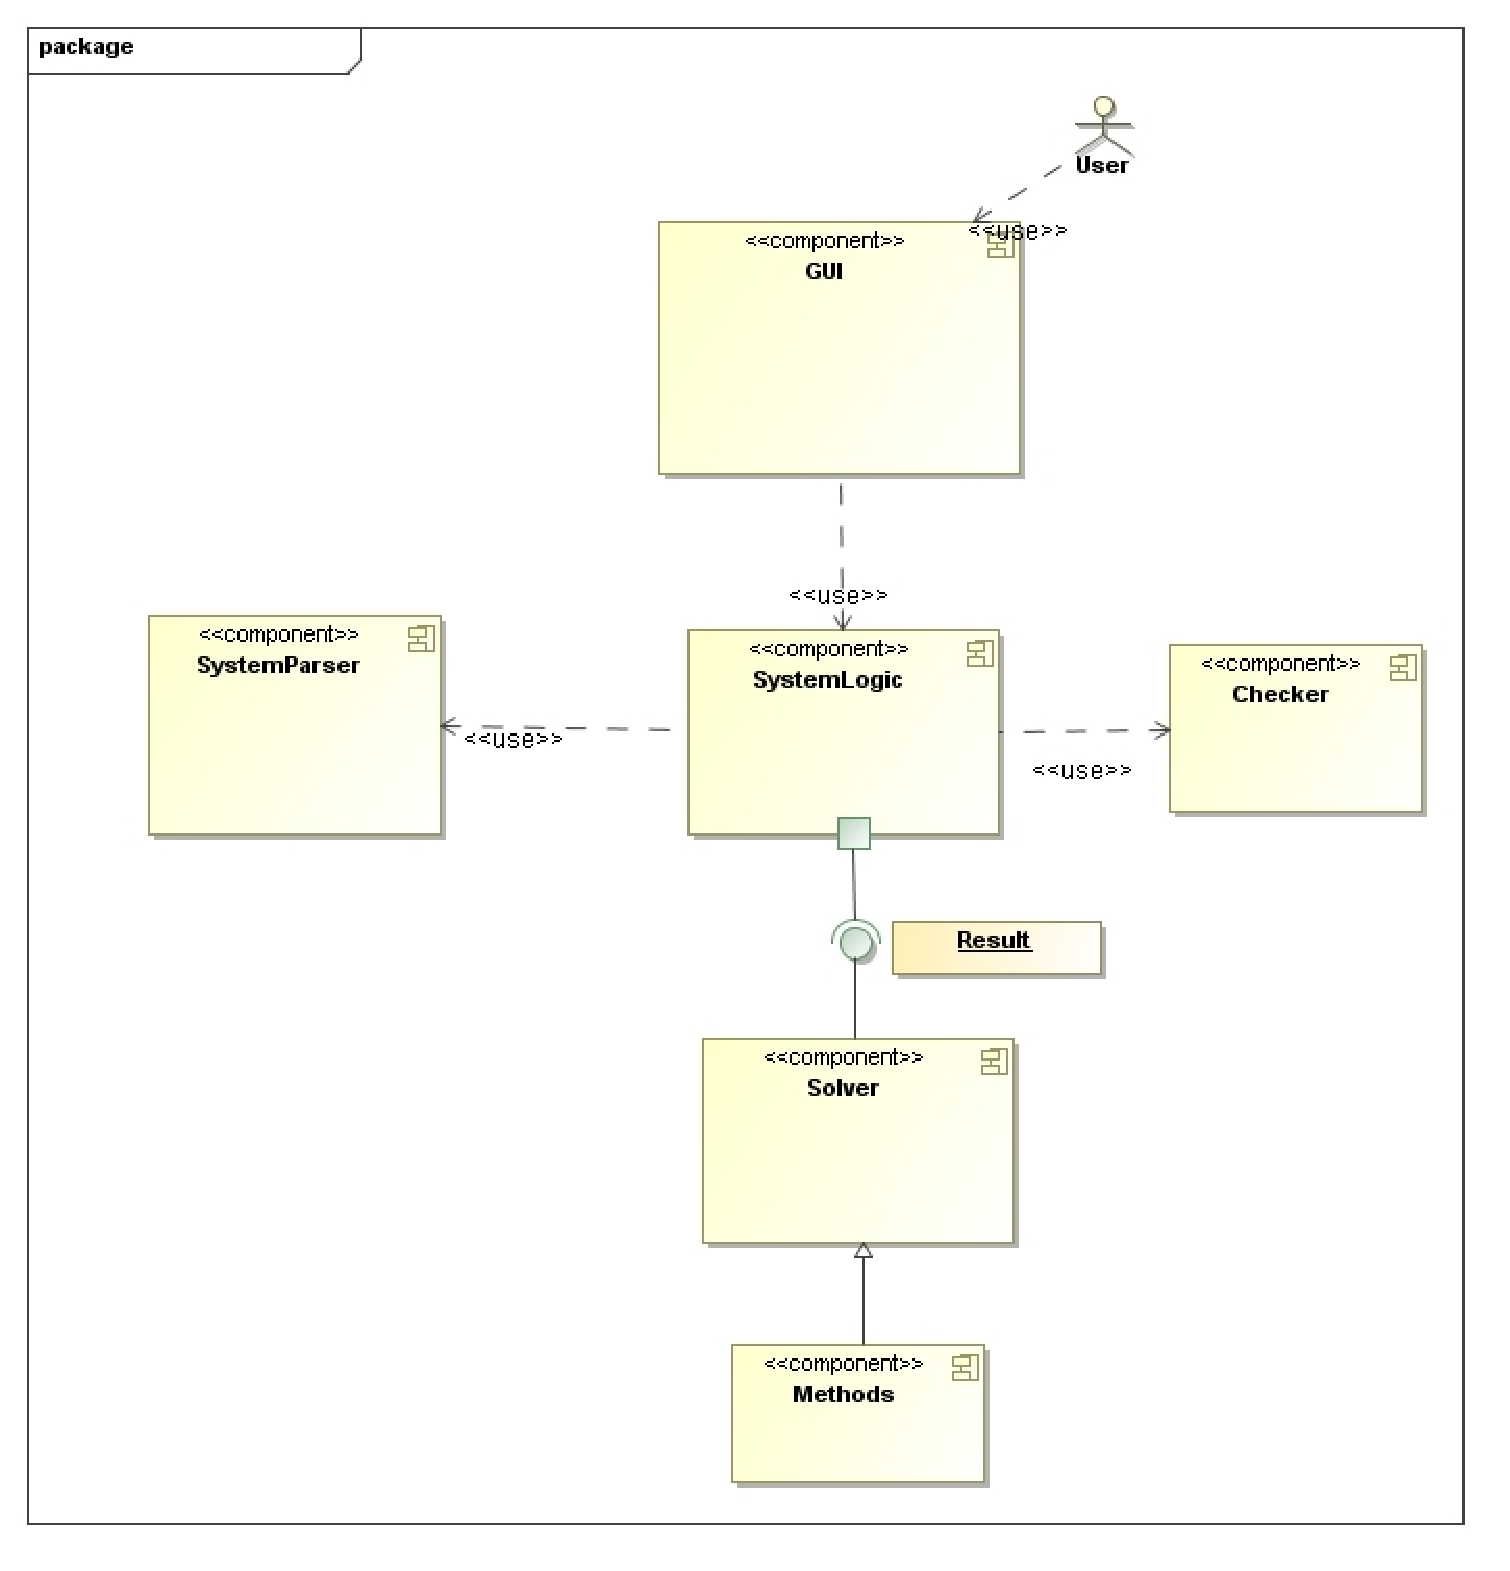
\includegraphics[width=\textwidth]{MSN1}
 % MSN1.jpg: 709x738 pixel, 72dpi, 25.01x26.03 cm, bb=0 0 709 738
 \caption{Arquitetura do Sistema}
 \label{fig:arquitetura}
\end{figure}


\subsection{Comunicação entre os módulos}

Interação dinâmica dos elementos é representada no diagrama de sequência da figura~\ref{fig:fluxo}. Cada elemento atua como as seguintes responsabilidades:

\begin{description}
 \item[Parser] Recebe como entrada um sistema em formato String, retorna um objeto ParsedSystem que representa o sistema após o parser;
 \item[Checke] Recebe o sistema representado através de duas matrizes, uma de coeficientes e outra de termos independentes. Retorna uma String que representa a classificação daquele sistema para definição de tipos de resolução;
 \item[Solver] Recebe as matrizes que compõem o sistema, o número de iterações, o valor estimado pelo usuário, a matriz de estimativas (para os métodos iterativos) e um objeto de Configuração. Este objeto Config contém possíveis configurações que são usados pelos métodos, por exemplo, se o método pode ser feito com ou sem pivoteamento;
 \item[Facade] A facade retorna um objeto Result que contém o passo a passo da resolução feita pelo método.
\end{description}

\begin{figure}[h]
 \centering
 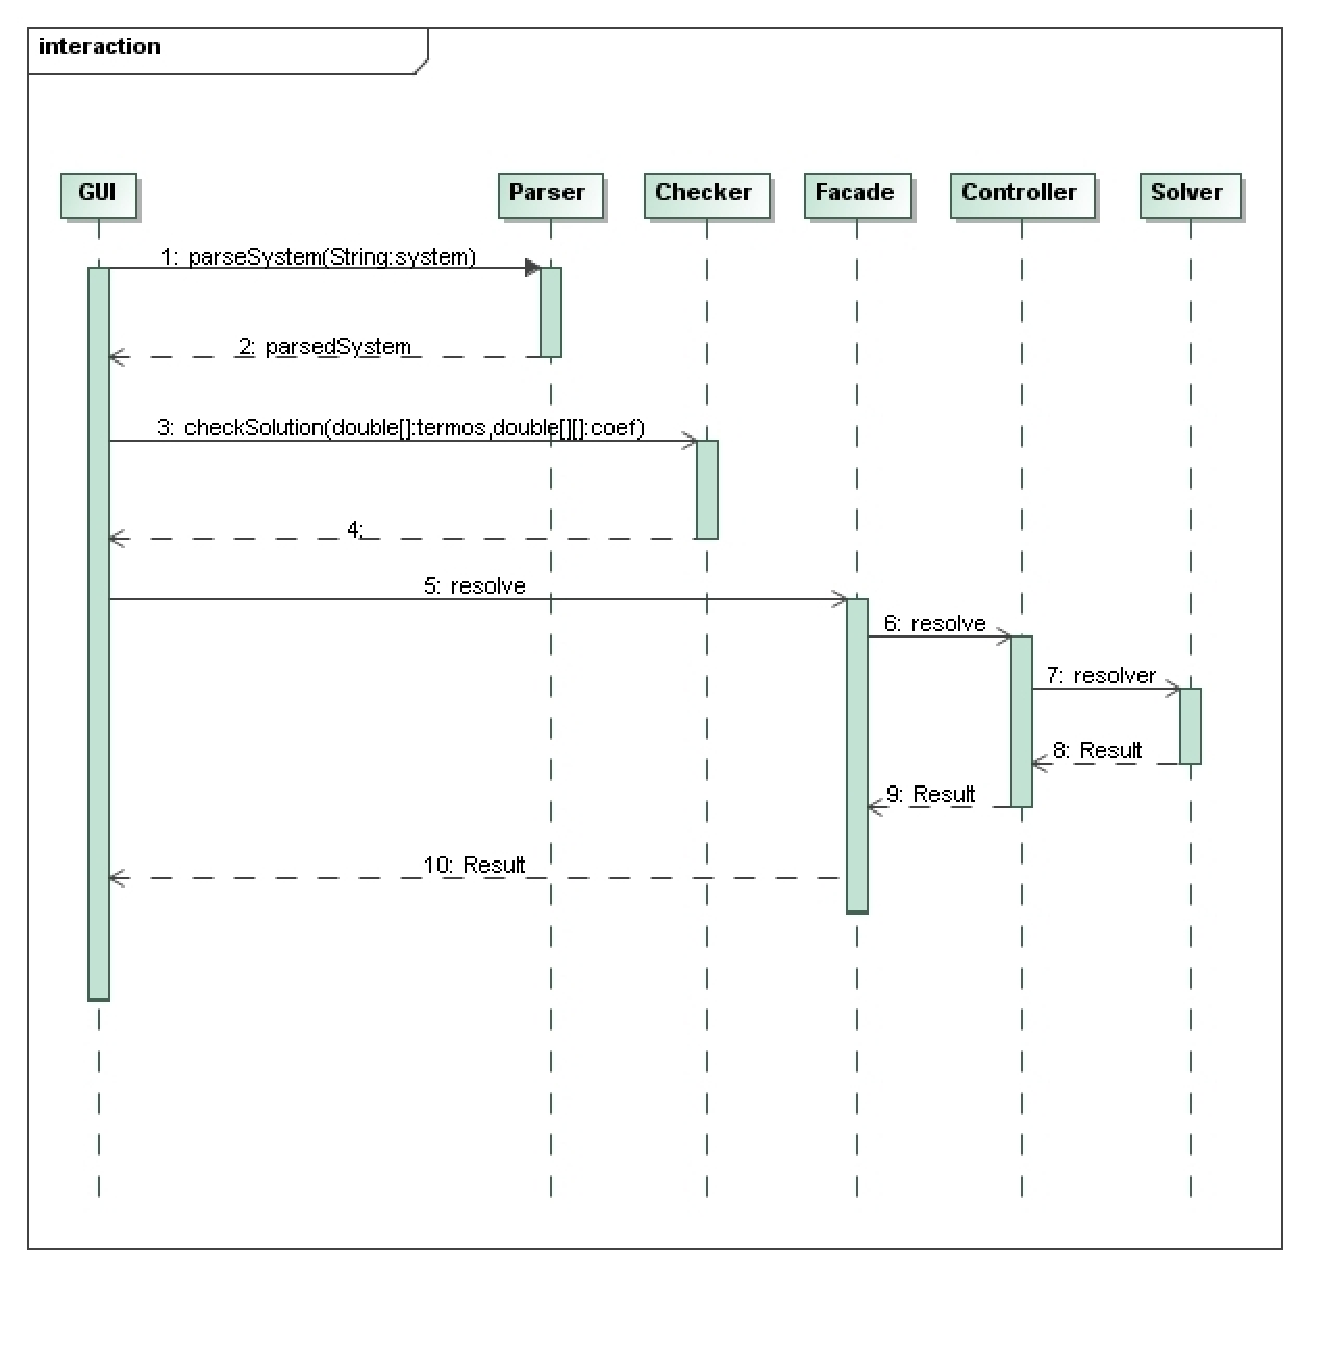
\includegraphics[width=\textwidth]{MSNFlow}
 % MSNFlow.jpg: 622x631 pixel, 72dpi, 21.94x22.26 cm, bb=0 0 622 631
 \caption{Fluxo de Execução do Sistema}
 \label{fig:fluxo}
\end{figure}

\section{Guia de Usabilidade da Interface}

Este guia levanta requisitos a serem usados na interface gráfica na forma de uma lista de fatores de usabilidade a serem adotados na construção da interface. 

\begin{itemize}
 \item Diálogo simples e claro 
 \item Linguagem do usuário
 \item Minimizar carga de memória
 \item Consistência
 \item Feedback
 \item Atalhos
 \item Documentação e ajuda
 \item Saídas claras
 \item Boas mensagens de erro
 \item Evitar erros
\end{itemize}

\bibliography{manual}

\end{document}
